\chapter{Conception}
\clearpage

\section{Introduction}
La phase de conception constitue une étape déterminante dans le cycle de développement logiciel. 
Elle permet de traduire les besoins fonctionnels identifiés en une architecture technique cohérente. 
Cette étape définit non seulement l'architecture globale et les composants principaux du système, 
mais aussi les interactions entre les différents modules.

Dans le cadre de ce projet, nous avons opté pour une approche intégrée où les fonctionnalités OptiHR et Gestion des Recours sont déployées au sein d'un portail d'applications unique, développé avec Laravel. Cette décision architecturale permet de mutualiser les composants techniques communs tout en offrant une expérience utilisateur cohérente et une maintenance simplifiée.

\section{Architecture du portail d'applications}

\subsection{Portail d'applications unifié}
Le portail d'applications constitue le point d'entrée unique du système et permet d'accéder aux différents modules fonctionnels (OptiHR et Gestion des Recours). Cette approche présente plusieurs avantages :

\begin{itemize}
    \item \textbf{Authentification unifiée} : Les utilisateurs s'authentifient une seule fois pour accéder à l'ensemble des fonctionnalités auxquelles ils ont droit.
    \item \textbf{Expérience utilisateur cohérente} : Interface graphique homogène à travers les différentes fonctionnalités.
    \item \textbf{Partage des composants communs} : Réutilisation des classes et services entre les modules.
    \item \textbf{Administration centralisée} : Gestion des utilisateurs, rôles et permissions au sein d'un système unique.
\end{itemize}

\begin{figure}[H]
    \centering
    \includegraphics[width=0.9\textwidth]{images/diagrammes/architecture/architecture-couches.pdf}
    \caption{Architecture en couches du portail d'applications}
    \label{fig:architecture_couches}
\end{figure}

\subsection{Architecture globale}
Le portail d'applications adopte une architecture en couches qui permet une séparation claire des responsabilités :

\begin{itemize}
    \item \textbf{Couche Présentation} : Interfaces utilisateur accessibles via navigateur web, incluant les templates Blade, les feuilles de style CSS et le code JavaScript.
    \item \textbf{Couche Application} : Logique métier et traitement des requêtes via les contrôleurs Laravel et les services métier.
    \item \textbf{Couche Persistance} : Stockage et récupération des données à travers l'ORM Eloquent et la base de données PostgreSQL.
\end{itemize}

Cette architecture en trois couches favorise la modularité et facilite la maintenance du code en isolant 
les changements à des zones spécifiques du système.

\subsection{Organisation structurelle du projet}
Le projet Laravel est organisé selon une structure modulaire qui permet de séparer clairement les fonctionnalités des deux applications tout en partageant les composants communs.
Cette organisation permet un développement modulaire où chaque équipe peut travailler indépendamment sur son module, tout en bénéficiant des composants partagés.

\subsection{Flux de données et interactions}
Les interactions entre les composants suivent un flux standardisé qui garantit la cohérence des opérations
et facilite le débogage :

\begin{figure}[H]
    \centering
    \includegraphics[width=0.9\textwidth]{images/diagrammes/architecture/flux-donnees.pdf}
    \caption{Flux de données dans le portail d'applications}
    \label{fig:flux_donnees}
\end{figure}

Le diagramme de séquence (figure \ref{fig:flux_donnees}) détaille le parcours d'une requête typique à travers les différentes couches du système :

\begin{enumerate}
    \item L'utilisateur interagit avec l'interface (Vue)
    \item Les requêtes sont acheminées vers le Contrôleur approprié
    \item Le Contrôleur délègue le traitement aux Services
    \item Les Services manipulent les données via le Modèle
    \item Le Modèle interagit avec la base de données
    \item Les données sont remontées à travers les couches
    \item L'interface est mise à jour avec les résultats
    \item Le résultat final est affiché à l'utilisateur
\end{enumerate}

\subsection{Authentification et autorisations}
Le module d'authentification et d'autorisation constitue un élément central du portail, permettant de :

\begin{itemize}
    \item Gérer les utilisateurs et leurs accès de manière centralisée
    \item Attribuer des rôles et permissions différents selon les modules
    \item Contrôler l'accès aux fonctionnalités via un système de middleware
\end{itemize}

Le système de rôles et permissions est conçu pour être granulaire, permettant d'accorder des droits spécifiques par module. Par exemple, un utilisateur pourrait avoir un rôle d'administrateur dans OptiHR mais un simple rôle de consultation dans Gestion des Recours.

\section{Technologies et outils}
Les outils et technologies suivants ont été utilisés pour la conception du
projet. Chaque outil est accompagné d'une description détaillée.

\renewcommand{\arraystretch}{1.5} % Espacement entre les lignes du tableau

\begin{center}
    \begin{table}[H]
        \begin{tabular}{|m{4cm}|m{10cm}|}
            \hline
            \textbf{Technologie}                                 & \textbf{Description}                                                                                                                                                                             \\
            \hline
            \includegraphics[width=3cm]{images/logo/uml.png}     & \textbf{UML} : Utilisé pour la modélisation des systèmes et la conception des structures du projet. Il permet de représenter graphiquement les différentes interactions et processus du système. \\
            \hline
            \includegraphics[width=3cm]{images/logo/modelio.png} & \textbf{Modelio} : Outil de modélisation UML permettant de créer des diagrammes tels que les diagrammes de classes, de séquence et d'activités.                                                  \\
            \hline
        \end{tabular}
        \caption{Tableau des technologies et outils utilisés pour la conception}
        \label{tab:technos_conception}
    \end{table}
\end{center}

\section{Module OptiHR}

\subsection{Découpage fonctionnel}
Le module OptiHR au sein du portail est subdivisé en plusieurs composants fonctionnels :

\begin{enumerate}
    \item \textbf{Gestion des employés} : Profils, informations personnelles et professionnelles
    \item \textbf{Gestion des absences} : Demandes de congés, workflow d'approbation et suivi
    \item \textbf{Gestion documentaire} : Bulletins de paie, documents administratifs et archivage
    \item \textbf{Communication interne} : Notes de service, alertes et notifications
\end{enumerate}


Cette organisation modulaire permet d'isoler les fonctionnalités et de faciliter les évolutions futures du système en minimisant les impacts entre composants.

\subsection{Modélisation des données}

\subsubsection{Diagramme conceptuel de données}
Le diagramme ci-dessous présente les principales entités du module OptiHR et leurs relations :

\begin{figure}[H]
    \centering
    \includegraphics[width=\textwidth]{images/diagrammes/class/diagramme.jpeg}
    \caption{Diagramme de classes du module OptiHR}
    \label{fig:class_diagram_optihr}
\end{figure}

\subsubsection{Entités principales}
Les entités clés du module OptiHR sont :

\begin{itemize}
    \item \textbf{Employee} : Informations personnelles et professionnelles des employés
    \item \textbf{Department} : Départements de l'organisation avec leurs hiérarchies
    \item \textbf{Job} : Postes et relations hiérarchiques
    \item \textbf{Absence} : Demandes de congés et d'absences avec leur workflow d'approbation
    \item \textbf{Note} : Communications internes et notes de service
    \item \textbf{File} : Documents administratifs et pièces jointes
\end{itemize}

\subsection{Circuit de validation des absences}
Un aspect essentiel du module OptiHR est le workflow de validation des demandes d'absence qui respecte la hiérarchie de l'ARCOP :

\begin{figure}[H]
    \centering
    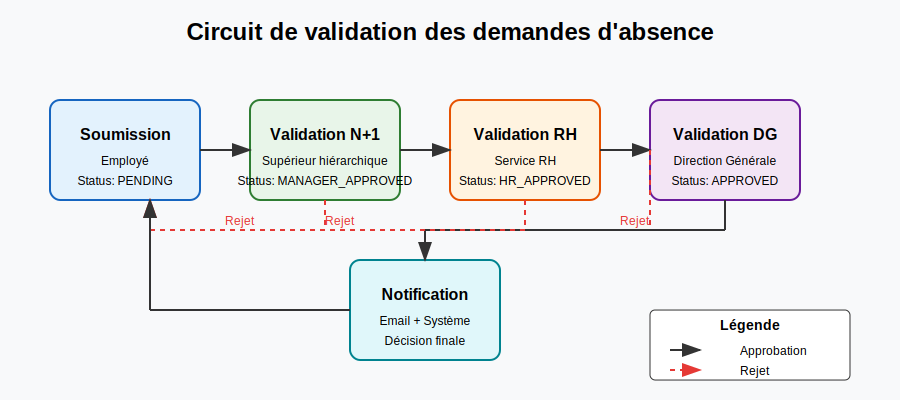
\includegraphics[width=0.9\textwidth]{images/diagrammes/architecture/workflow-validation-svg.pdf}
    \caption{Circuit de validation des demandes d'absence}
    \label{fig:workflow_validation}
\end{figure}

Ce workflow garantit que chaque demande d'absence suit un parcours de validation conforme à l'organisation hiérarchique de l'ARCOP, avec des statuts clairement définis à chaque étape du processus.

\section{Module Gestion des Recours}

\subsection{Découpage fonctionnel}
Le module Gestion des Recours comprend les composants fonctionnels suivants :

\begin{enumerate}
    \item \textbf{Enregistrement des recours} : Saisie et suivi des recours déposés
    \item \textbf{Traitement des dossiers} : Processus d'analyse et de décision
    \item \textbf{Reporting et statistiques} : Tableaux de bord et indicateurs de performance
    \item \textbf{Alertes et notifications} : Suivi des délais et rappels
\end{enumerate}

\subsection{Modélisation des données}

\subsubsection{Diagramme conceptuel de données}
Le diagramme suivant présente les principales entités du module Gestion des Recours et leurs relations :

\begin{figure}[H]
    \centering
    \includegraphics[width=\textwidth]{images/diagrammes/class/Diagramme de classe recours.png}
    \caption{Diagramme de classes du module Gestion des Recours}
    \label{fig:class_diagram_recours}
\end{figure}

\subsubsection{Entités principales}
Les entités clés du module Gestion des Recours sont :

\begin{itemize}
    \item \textbf{Appeal} : Recours déposés avec leurs caractéristiques et statuts
    \item \textbf{Applicant} : Requérants ayant déposé des recours
    \item \textbf{Authority} : Autorités contractantes concernées par les recours
    \item \textbf{Dac} : Dossiers d'Appel à Concurrence liés aux recours
    \item \textbf{Decision} : Décisions rendues suite à l'analyse des recours
\end{itemize}

\subsection{Processus de traitement des recours}
Le traitement d'un recours suit un processus précis qui comprend les étapes suivantes :

\begin{enumerate}
    \item \textbf{Réception et enregistrement} : Saisie des informations du recours
    \item \textbf{Analyse de recevabilité} : Vérification des critères formels
    \item \textbf{Étude au fond} : Analyse détaillée du dossier
    \item \textbf{Prise de décision} : Délibération et établissement de la décision
    \item \textbf{Notification} : Information des parties concernées
    \item \textbf{Archivage} : Conservation du dossier avec sa décision
\end{enumerate}

Ce processus est accompagné d'un système d'alertes qui signale les dépassements de délais réglementaires pour garantir le traitement dans les temps impartis.

\section{Intégration et points de convergence}

\subsection{Composants partagés}
Plusieurs composants du portail sont partagés entre les deux modules fonctionnels :

\begin{itemize}
    \item \textbf{Système d'authentification} : Gestion unifiée des utilisateurs et connexions
    \item \textbf{Moteur de notifications} : Système d'alertes et de notifications
    \item \textbf{Gestionnaire de documents} : Stockage et récupération des fichiers
    \item \textbf{Interface utilisateur} : Composants UI réutilisables (dashboard, tableaux, formulaires)
    \item \textbf{Services utilitaires} : Journalisation, gestion des dates, formatage, etc.
\end{itemize}

\subsection{Points d'intégration}
Bien que les deux modules gèrent des processus métier distincts, certains points d'intégration ont été identifiés :

\begin{itemize}
    \item \textbf{Tableau de bord unifié} : Vue d'ensemble combinant les indicateurs des deux modules
    \item \textbf{Notifications consolidées} : Centre de notifications regroupant les alertes des deux modules
    \item \textbf{Recherche globale} : Possibilité de rechercher dans les deux modules simultanément
    \item \textbf{Rapports croisés} : Possibilité de générer des rapports combinant des données des deux modules
\end{itemize}

\section{Considérations techniques}

\subsection{Déploiement et environnements}
Le portail d'applications est conçu pour être déployé sur l'infrastructure interne de l'ARCOP selon une stratégie à plusieurs environnements :

\begin{itemize}
    \item \textbf{Environnement de développement} : Pour le développement actif et les tests unitaires
    \item \textbf{Environnement de test} : Pour les tests d'intégration et les validations fonctionnelles
    \item \textbf{Environnement de production} : Pour l'utilisation par les utilisateurs finaux
\end{itemize}

\subsection{Performance et scalabilité}
Pour garantir des performances optimales du portail, plusieurs techniques sont mises en œuvre :

\begin{itemize}
    \item \textbf{Mise en cache} : Utilisation du système de cache de Laravel pour les données fréquemment consultées
    \item \textbf{Optimisation des requêtes} : Utilisation judicieuse des eager loading pour réduire le nombre de requêtes
    \item \textbf{Pagination} : Limitation des résultats par page pour les listes volumineuses
    \item \textbf{Traitements asynchrones} : Utilisation des queues Laravel pour les tâches lourdes (génération de rapports, envoi massif de notifications)
\end{itemize}

\subsection{Sécurité}
La sécurité du portail est assurée par plusieurs mécanismes :

\begin{itemize}
    \item \textbf{Authentification robuste} : Utilisation de Laravel Sanctum avec politique de mots de passe forts
    \item \textbf{Autorisations granulaires} : Système de rôles et permissions précis avec vérifications à plusieurs niveaux
    \item \textbf{Protection CSRF} : Jetons CSRF pour toutes les requêtes POST
    \item \textbf{Validation des entrées} : Validation côté serveur de toutes les données entrantes
    \item \textbf{Journalisation} : Traçabilité des actions sensibles pour faciliter les audits
\end{itemize}

\section{Conclusion}
La conception d'un portail d'applications unique intégrant les modules OptiHR et Gestion des Recours représente une approche optimale pour répondre aux besoins de l'ARCOP. Cette architecture offre plusieurs avantages significatifs :

\begin{itemize}
    \item \textbf{Cohérence technique} : Utilisation des mêmes technologies et pratiques de développement
    \item \textbf{Expérience utilisateur unifiée} : Interface homogène et navigation fluide entre les modules
    \item \textbf{Efficacité opérationnelle} : Authentification unique et partage des composants communs
    \item \textbf{Maintenance simplifiée} : Base de code centralisée facilitant les évolutions et corrections
\end{itemize}

Cette approche intégrée, tout en conservant une séparation logique des préoccupations métier, permettra à l'ARCOP de disposer d'une solution moderne, évolutive et parfaitement adaptée à ses processus organisationnels.

\clearpage